%!TeX root=../tese.tex
%("dica" para o editor de texto: este arquivo é parte de um documento maior)
% para saber mais: https://tex.stackexchange.com/q/78101

\chapter{Metodologia}

Neste trabalho, utilizou-se dados públicos de fontes como o Instituto Brasileiro 
de Geografia e Estatística (IBGE), a Fundação Getúlio Vargas, FGV, e o 
Banco Central do Brasil (BACEN) para prever o consumo mensal de 
cimento nos estados da União. Para melhorar o desempenho dos modelos de 
aprendizado de máquina, realizaram-se técnicas
de preparação de dados, como o preenchimento de valores nulos, e para mensurar 
o acerto das previsões são aplicadas as métricas estatísticas: \textit {root 
mean squared error} (RMSE),  \textit{mean absolute error} (MAE) e \textit{mean 
absolute percentage error} (MAPE), além do delta percentual.


\section{Dados}


O consumo mensal de cimento nos estados do Brasil, alvo da previsão 
dos modelos aplicados neste trabalho, é um indicador fornecido pelo SNIC, 
Sindicato Nacional da Indústria de Cimento. Os dados obtidos apresentavam granularidade
mensal para cada um dos estados da União e estavam disponíveis de 1990 até 2019,
a exceção dos anos de 2001 e 2002. Dessa forma, optou-se por utilizar apenas 
dados posteriores a 2003 no trabalho, uma vez que os modelos recorrentes se 
valem do contexto para obter a próxima previsão \ref{rnn} , então esse lapso nos dados
poderia trazer inconsistências no modelo.

Além disso, o descarte de dados mais antigos favorece a assertividade do 
modelo, pois houve alteração no total de cimento consumida no Brasil
ao longo do tempo, então dados mais antigos poderiam privilegiar tendências 
mais antigas. Retirar dados mais antigos, então evita, por exemplo, que a 
estagnação econômica da época de hiperinflação ou o otimismo do Plano real
impacto a previsão atual. Essa alteração na quantidade de cimento consumida pela União
pode ser observada na imagem abaixo. 

\begin{figure}[H] 
    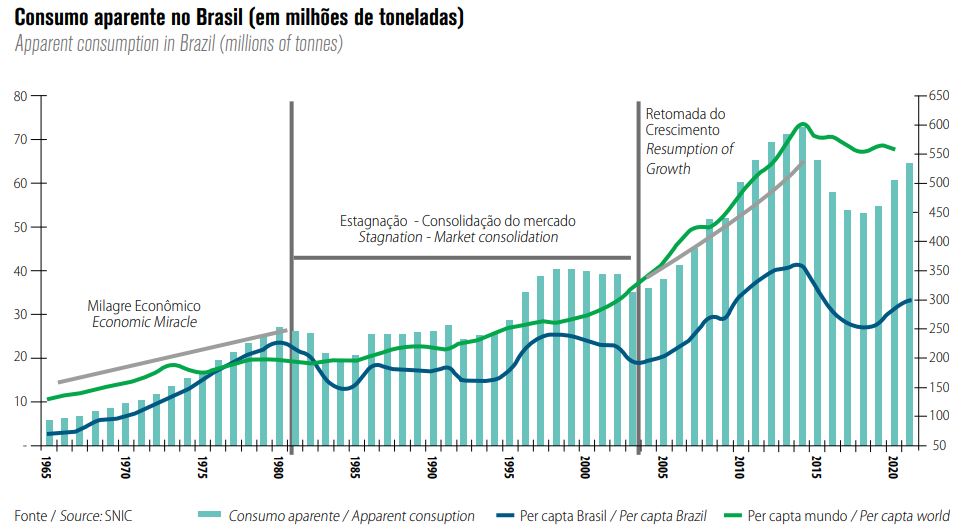
\includegraphics[width= 14cm]{../figuras/evolucao-consumo.png}
    \caption{Evolução do consumo de cimento no Brasil \cite{relatorio-snic}}
    \label{fig:evolucao-consumo-cimento}
\end{figure}

Observa-se, por exemplo, uma queda no consumo de cimento entre 2015 e 2018,
fruto das crises econômicas nesse período.
Alem disso, a tendência do consumo não é única para os estados. 

\begin{figure}[H]
    \centering
    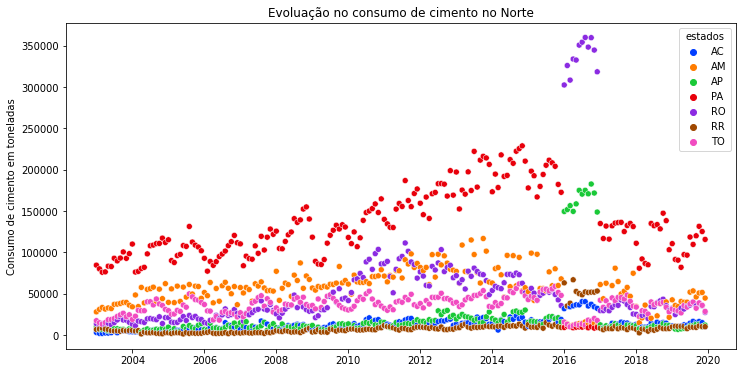
\includegraphics[width=6cm]{../figuras/evolucao-consumo-norte.png}
    \caption{Consumo de cimento no Norte}
\end{figure}


% \begin{figure}[H]
%     \centering
%     \begin{subfigure}{0.6 \textwidth}
%         \centering
%         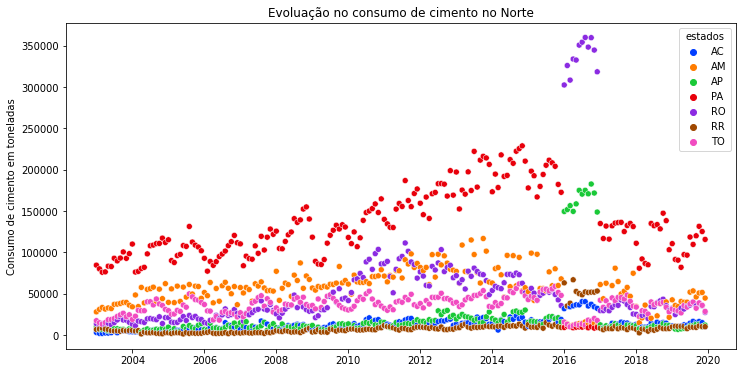
\includegraphics[width=6cm]{../figuras/evolucao-consumo-norte.png}
%         \caption{Consumo de cimento no Norte}
%     \end{subfigure}
%     \hfill
%     \begin{subfigure}{0.6 \textwidth}
%         \centering
%         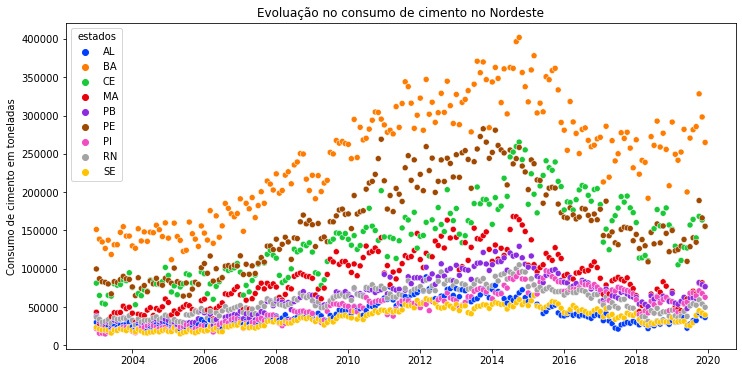
\includegraphics[width=6cm]{../figuras/evolucao-consumo-nordeste.png}
%         \caption{Consumo de cimento no Nordeste}
%     \end{subfigure}
% \end{figure}
    


\begin{table}[H]
    \centering
    \caption{Indicadores de crescimento econômico}
    \begin{tabular}{llll}
        \toprule
        Indicador                   & Fonte & Período disponível & Granularidade         \\
        \midrule
        PIB a preços constantes     & IBGE  & 1983 até 2019      & anual por estado      \\
        PIB a preços de mercado     & IBGE  & 1985 ate 2019      & anual por estado      \\
        PIB per capita              & IBGE  & 1985 até 2019      & anual por estado      \\
        PIB da construção civil     & IBGE  & 1985 até 2019      & anual por estado      \\
        Desemprego                  & IBGE  & 1991 até 2022      & anual por estado até 2014 e mensal para o Brasil a partir de 2012      \\
        \bottomrule
    \end{tabular}
\end{table}

\begin{table}[H]
    \centering
    \caption{Indicadores de inflação e política monetária}
    \begin{tabular}{llll}
        \toprule
        Indicador                   & Fonte & Período disponível & Granularidade         \\
        \midrule
        IPCA                        & IBGE  & 1981 até 2021      & mensal para o Brasil      \\
        INCC                        & FGV   & 1980 ate 2021      & mensal para o Brasil      \\
        IGP                         & FGV   & 1944 até 2021      & mensal para o Brasil      \\
        SELIC                       & IBGE  & 1986 até 2022      & mensal para o Brasil      \\
        \bottomrule
    \end{tabular}
\end{table}

\begin{table}[H]
    \centering
    \caption{Indicadores de inflação e política fiscal}
    \begin{tabular}{llll}
        \toprule
        Indicador                   & Fonte & Período disponível & Granularidade         \\
        \midrule
        NFSP                        & BACEN  & 1991 até 2022      & mensal para o Brasil      \\
        estoque de dívida pública   & IPEA   & 1947 ate 2019      & anual para o Brasil      \\
        \bottomrule
    \end{tabular}
\end{table}

\begin{table}[H]
    \centering
    \caption{Indicadores sociais}
    \begin{tabular}{llll}
        \toprule
        Indicador                   & Fonte & Período disponível & Granularidade         \\
        \midrule
        População                   & IBGE   & 1991 até 2021      & anual por estado      \\
        IDH                         & IBGE   & 1991 ate 2017      & irregular      \\
        \bottomrule
    \end{tabular}
\end{table}


\begin{table}[H]
    \centering
    \caption{Indicadores de construção civil}
    \begin{tabular}{llll}
        \toprule
        Indicador                   & Fonte & Período disponível & Granularidade         \\
        \midrule
        Produção mensal de cimento  & SNIC  & 2003 até 2022      & mensal por estado      \\
        Valor médio do cimento Portland em reais por quilograma   & IPEA   & 1947 ate 2019      & anual para o Brasil      \\
        \bottomrule
    \end{tabular}
\end{table}

Com o objetivo de direcionar a estratégia de preparação de dados
foi realizada uma análise exploratória de cada um dos dados de 
entrada e da variável resposta. Destaca-se nessa análise, a alta
taxa de variação dos dados de entrada, em alguns indicadores, por exemplo 
para o  PIB da construção civil, 
o desvio padrão é maior que o valor médio do indicador. Esse comportamento 
se deve a estados com valores discrepantes em relação ao resto do país.
A partir dessa análise, 
optou-se por utilizar os dados de 2003 até 2019 para o estudo.

Foram adotadas estratégias para garantir dados na granularidade
mensal e por estado. Caso os indicadores apresentassem granularidade anual, 
o valor foi dividido por 12 de modo a obter a média mensal, já caso a granularidade
fosse a nível de Brasil, o valor apresentado foi repetido para todos os 
estados.


A estratégia utilizada para lidar com dados faltantes foi, sempre que possível,
repetir o valor anterior que estava disponível nos dados de entrada para
preencher a ocorrência. Contudo, alguns indicadores não apresentavam 
valores mais antigos, então foi usado um valor não presente no intervalo
de dados de entrada para marcar como nulo.

Além disso, tomou-se um cuidado para evitar que a previsão fosse 
realizada com os dados do mês anterior ou do ano anterior no caso dos
indicadores anuais. Deslocou-se, portanto, os dados de entrada 
para frente em um ocorrência de modo a associar os dados de um 
mês com o consumo no mês seguinte.\footnote{os dados correspondentes 
a, por exemplo, fevereiro de 2004 estão relacionados ao consumo de 
cimento em março de 2004, com o objetivo de propor um cenário mais pertinente, 
uma vez que o objetivo do projeto é prever a demanda por cimento no mês seguinte 
em um estado a partir dos dados do mês atual e, eventualmente, dos anteriores.
}

Por fim, o estado correspondente à medição foi usado como dado de entrada. 
Como os modelos de inteligência artificial aceitam apenas caracteres numéricos,
utilizou-se o método de codificação \textit{one hot} para criar 27 colunas, uma
para cada estado, nas quais o valor é 1 quando a linha possui dados daquele estado 
e é 0 caso contrário.


    \section{Avaliação de performance}

    Para comparar a eficiência dos modelos mede-se os erros de 
    cada previsão, ou seja, a distância entre o valor previsto 
    pelo algoritmo e o valor do dado real. Neste trabalho, 
    utilizou-se as seguintes métricas estatísticas para 
    mensurar o desempenho: \textit{mean absolute error} (MAE),
    \textit{root mean square  error} (RMSE) e \textit{mean 
    absolute percentage error} (MAPE). Além disso, foi utilizado
    o delta percentual ($\Delta$) para avaliar se o modelo tende 
    a subestimar ou superestimar o valor previsto, se é otimista
    ou pessimista.

\subsection{Mean absolute error (MAE)}

    O MAE, sigla do inglês para \textit{mean absolute error}
    ou média do erro absoluto mede o erro absoluto de cada previsão
    e é dado por:\cite{forecast-evaluation-ds}

    \begin{equation}
        MAE = \frac{\sum_{i=1}^n |\hat{y}_i - y_i|}{n}
    \end{equation}

\subsection{Root mean squared error (RMSE)}

    A RMSE, sigla para \textit{root mean squared  error} é
    semelhante à MAE, contudo eleva os erros ao quadrado antes de 
    somá-los e tira aa raiz logo depois. A RMSE é, por tanto, 
    mais sensível a \textit{outliers}.\cite{forecast-evaluation-ds}

    \begin{equation}
        RMSE = \sqrt{\frac{\sum_{i=1}^n (\hat{y}_i - y_i)^2}{n}}
    \end{equation}

\subsection{Mean absolute percentage error (MAPE)}

    Foi utilizada também a MAPE, \textit{Mean absolute
    percentage error}, para mensurar a escala do erro em 
    relação ao tamanho das medições.

    \begin{equation}
        MAPE=\sum_{t=1}^n\left|\frac{y_t-\hat{y}_t}{y_t}\right|
    \end{equation}

\subsection{Delta percentual}

O delta percentual, $\Delta$, é utilizado para mensurar se o 
modelo apresenta tendência de subestimar ou superestimar a variável, se 
é otimista ou pessimista.

\begin{equation}
    \Delta = \frac{\hat{y_i} - y_i}{y_i}
\end{equation}